\begin{minipage}{0.45\textwidth}
  % Code Listing
  \begin{lstlisting}[style=Cstyle]
void triangleBranch(int condition) {
    // EBB: Entry Basic Block
    x_ ++;
    if (x == 0) {
        // TBB: True Block
        x_ = 42;
    }
    // FBB: Fall-through Block
    y_ = 100; // Common operation
}
  \end{lstlisting}
  \end{minipage}%
  \hfill
  \begin{minipage}{0.5\textwidth}
  \centering
  % Triangle Branch Diagram
  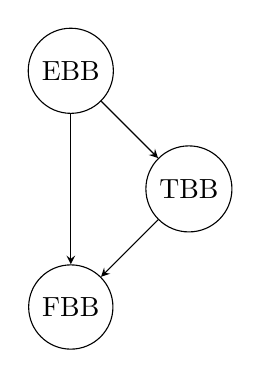
\begin{tikzpicture}[node distance=1.5cm and 2cm, >=stealth]
      % Nodes
      \node[circle, draw, fill=white, minimum size=0.8cm] (EBB) at (0, 3) {EBB};
      \node[circle, draw, fill=white, minimum size=0.8cm] (TBB) at (1.5, 1.5) {TBB};
      \node[circle, draw, fill=white, minimum size=0.8cm] (FBB) at (0, 0) {FBB};

      % Edges
      \draw[->] (EBB) -- (TBB);
      \draw[->] (EBB) -- (FBB);
      \draw[->] (TBB) -- (FBB);
  \end{tikzpicture}
  \end{minipage}
